\documentclass[12pt,a4paper,reqno]{amsart}

% language
\usepackage[greek,english]{babel}
\usepackage[utf8]{inputenc}
\usepackage{alphabeta}

% change default names to greek
\addto\captionsenglish{
    \renewcommand{\contentsname}{Περιεχόμενα}
    \renewcommand{\refname}{Βιβλιογραφία}
    \renewcommand{\datename}{Ημερομηνία:}
    \renewcommand{\urladdrname}{Ιστοσελίδα}
}

% math 
\usepackage{amsmath,amsthm,amssymb,amscd}

% font
\usepackage[cal=euler]{mathalfa}
\usepackage{libertinus-type1}
% \usepackage{txfonts} % for upright greek letters
\usepackage{bm} % for bold symbols
\usepackage{bbm} % for the simply-looking bb symbols

% miscellaneous 
\usepackage{changepage} %for indenting environments
\usepackage{csquotes} % example: \textcquote{}
\usepackage{blkarray}
\setcounter{MaxMatrixCols}{20} % default for pmatrix is 10!!
\usepackage{ytableau}
\usepackage{array} %needed to increase the vertical length in a tabular

% drawing
\usepackage{tikz,tikz-cd}
\usetikzlibrary{shapes.misc, patterns, matrix, calc, intersections,positioning}
\usepackage{graphics,graphicx}
\usepackage{float} % provides enhanced control and customization options for floating objects such as figures and tables

% colors
\usepackage{xcolor}
\definecolor{darkcandyapplered}{rgb}{0.64, 0.0, 0.0}
\definecolor{midnightblue}{rgb}{0.1, 0.1, 0.44}
\definecolor{mylightblue}{HTML}{336699}
\definecolor{burntorange}{rgb}{0.8, 0.33, 0.0}
\definecolor{iceberg}{rgb}{0.44, 0.65, 0.82}
\definecolor{applegreen}{rgb}{0.55, 0.71, 0.0}
\definecolor{canaryyellow}{rgb}{1.0, 0.94, 0.0}

% hrefs
\usepackage{hyperref}
\usepackage[noabbrev,capitalize]{cleveref}
\hypersetup{
    pdftoolbar=true,        
    pdfmenubar=true,        
    pdffitwindow=false,     
    pdfstartview={FitH},  % fits the width of the page to the window
    pdftitle={},
    pdfauthor={},
    pdfsubject={},
    pdfkeywords={},
    pdfnewwindow=true,  % links in new window
    colorlinks=true,  % false: boxed links; true: colored links
    linkcolor=darkcandyapplered,   % color of internal links
    citecolor=midnightblue,  % color of links to bibliography
    urlcolor=cyan,  % color of external links
    linktocpage=true  % changes the links from the section body to the page number
    }

% geometry
\textwidth=16cm 
\textheight=21cm 
\hoffset=-55pt 
\footskip=25pt

% thm envs (you might need to change the path)
\theoremstyle{definition}
\newtheorem{theorem}{Θεώρημα}
\newtheorem{proposition}[theorem]{Πρόταση}
\newtheorem{lemma}[theorem]{Λήμμα}
\newtheorem{corollary}[theorem]{Πόρισμα}
\newtheorem{conjecture}[theorem]{Εικασία}
\newtheorem{problem}[theorem]{Πρόβλημα}
\newtheorem*{claim}{Ισχυρισμός}
\newtheorem{observation}[theorem]{Παρατήρηση}
\newtheorem{definition}[theorem]{Ορισμός}
\newtheorem{question}[theorem]{Ερώτημα}
\newtheorem*{questions}{Ερωτήματα}
\newtheorem*{que}{Ερώτημα}
\newtheorem{example}[theorem]{Παράδειγμα}
\newtheorem{exercise}{Άσκηση}

\theoremstyle{remark}
\newtheorem*{remark}{Παρατήρηση}

% fixes the correct numbering of environments
\numberwithin{theorem}{section}
\numberwithin{exercise}{section}
\numberwithin{equation}{section}

% math ops 
% fields
\newcommand{\NN}{\mathbbmss{N}} 
\newcommand{\ZZ}{\mathbbmss{Z}} 
\newcommand{\QQ}{\mathbbmss{Q}} 
\newcommand{\RR}{\mathbbmss{R}} 
\newcommand{\CC}{\mathbbmss{C}} 
\newcommand{\KK}{\mathbbmss{K}} 
\newcommand{\FF}{\mathbbmss{F}} 
\newcommand{\HH}{\mathbbmss{H}} 

% symmetric group
\newcommand{\fS}{\mathfrak{S}}  

% calligraphic 
\newcommand{\aA}{\mathcal{A}} 
\newcommand{\bB}{\mathcal{B}}
\newcommand{\cC}{\mathcal{C}}
\newcommand{\dD}{\mathcal{D}}
\newcommand{\eE}{\mathcal{E}}
\newcommand{\fF}{\mathcal{F}}
\newcommand{\hH}{\mathcal{H}}
\newcommand{\iI}{\mathcal{I}}
\newcommand{\lL}{\mathcal{L}}
\newcommand{\oO}{\mathcal{O}}
\newcommand{\pP}{\mathcal{P}}
\newcommand{\sS}{\mathcal{S}}
\newcommand{\mM}{\mathcal{M}}
\newcommand{\uU}{\mathcal{U}}

% bold
\newcommand{\bfa}{\mathbf{a}}
\newcommand{\bfe}{\mathbf{e}}
\newcommand{\bfF}{\pmb{F}}
\newcommand{\bfR}{\pmb{R}}
\newcommand{\bfv}{\mathbf{v}}
%\newcommand{\bfx}{\bm{x}}
%\newcommand{\bfx}{\mathbf{x}} 
\newcommand{\bfx}{\pmb{x}}
\newcommand{\bfX}{\pmb{X}}
\newcommand{\bfy}{\pmb{y}}
\newcommand{\bfz}{\pmb{z}}

% roman
\newcommand{\rmA}{\mathrm{A}}
\newcommand{\rmB}{\mathrm{B}}
\newcommand{\rmC}{\mathrm{C}}
\newcommand{\rmD}{\mathrm{D}} 
\newcommand{\rmH}{\mathrm{H}} 
\newcommand{\rmh}{\mathrm{h}} 
\newcommand{\rmI}{\mathrm{I}} 
\newcommand{\rmK}{\mathrm{K}}
\newcommand{\rmM}{\mathrm{M}}
\newcommand{\rmP}{\mathrm{P}}  
\newcommand{\rmp}{\mathrm{p}}  
\newcommand{\rmQ}{\mathrm{Q}}  
\newcommand{\rmR}{\mathrm{R}}
\newcommand{\rmS}{\mathrm{S}}
\newcommand{\rmT}{\mathrm{T}}
\newcommand{\rmU}{\mathrm{U}}
\newcommand{\rmV}{\mathrm{V}}
\newcommand{\rmY}{\mathrm{Y}}
\newcommand{\rmZ}{\mathrm{Z}}
\newcommand{\rmz}{\mathrm{z}}

% arrows and symbols 
\renewcommand{\to}{\rightarrow}
\newcommand{\toto}{\longrightarrow}
\newcommand{\mapstoto}{\longmapsto}
\newcommand{\then}{\Rightarrow}
\newcommand{\IFF}{\Leftrightarrow}
\newcommand{\tl}{\tilde}
\newcommand{\wtl}{\widetilde}
\newcommand{\ol}{\overline}
\newcommand{\ul}{\underline}
\newcommand{\oldemptyset}{\emptyset}
\renewcommand{\emptyset}{\varnothing}
\DeclareMathSymbol{\Arg}{\mathbin}{AMSa}{"39} % for arguments 
\newcommand{\onto}{\ensuremath{\twoheadrightarrow}}
\newcommand{\tle}{\trianglelefteq}
\newcommand{\tge}{\trianglerighteq}

% custom ops
\newcommand{\rmKer}{\mathrm{Ker}}
\newcommand{\rmIm}{\mathrm{Im}}
\newcommand{\lcm}{\mathrm{lcm}}

% absolute value symbol
\usepackage{mathtools} 
\DeclarePairedDelimiter\abs{\lvert}{\rvert}%
\DeclarePairedDelimiter\norm{\lVert}{\rVert}%
\makeatletter
\let\oldabs\abs
\def\abs{\@ifstar{\oldabs}{\oldabs*}}

% tensor symbol
\newcommand{\tensor}[1]{%
  \mathbin{\mathop{\otimes}\limits_{#1}}%
}

% permutation cycle notation
\ExplSyntaxOn
\NewDocumentCommand{\cycle}{ O{\;} m }
 {
  (
  \alec_cycle:nn { #1 } { #2 }
  )
 }

\seq_new:N \l_alec_cycle_seq
\cs_new_protected:Npn \alec_cycle:nn #1 #2
 {
  \seq_set_split:Nnn \l_alec_cycle_seq { , } { #2 }
  \seq_use:Nn \l_alec_cycle_seq { #1 }
 }
\ExplSyntaxOff

% setminus symbol
\newcommand{\mysetminusD}{\hbox{\tikz{\draw[line width=0.6pt,line cap=round] (3pt,0) -- (0,6pt);}}}
\newcommand{\mysetminusT}{\mysetminusD}
\newcommand{\mysetminusS}{\hbox{\tikz{\draw[line width=0.45pt,line cap=round] (2pt,0) -- (0,4pt);}}}
\newcommand{\mysetminusSS}{\hbox{\tikz{\draw[line width=0.4pt,line cap=round] (1.5pt,0) -- (0,3pt);}}}
\newcommand{\sm}{\mathbin{\mathchoice{\mysetminusD}{\mysetminusT}{\mysetminusS}{\mysetminusSS}}}

% miscellaneous commands
\newcommand{\defn}[1]{{\color{mylightblue}{#1}}}
\newcommand{\toDo}{{\bf\color{red} TODO}}
\newcommand{\toCite}{{\bf\color{green} CITE}}
\newcommand*{\vertbar}{\rule[-1ex]{0.5pt}{2.5ex}} % for matrices with column vectors
\newcommand*{\horzbar}{\rule[.5ex]{2.5ex}{0.5pt}} % for matrices with row vectors
\newcommand{\myblue}[1]{{\color{iceberg}{#1}}}
\newcommand{\myorange}[1]{{\color{burntorange}{#1}}}
\newcommand{\mygreen}[1]{{\color{applegreen}{#1}}}
\newcommand{\myred}[1]{{\color{darkcandyapplered}{#1}}}

% ferrer's diagram
\newcommand{\fdiagram}[1]{
    \begin{tikzpicture}[scale=.7]
        \fill foreach \Z [count=\Y] in {#1}
        {foreach \X in {1,...,\Z} 
        {(\X,-\Y) circle[radius=3pt]}};
    \end{tikzpicture}
}

%
\makeatletter
\def\mathcolor#1#{\@mathcolor{#1}}
\def\@mathcolor#1#2#3{%
  \protect\leavevmode
  \begingroup
    \color#1{#2}#3%
  \endgroup
}
\makeatother

% 
\newenvironment{nouppercase}{%
  \let\uppercase\relax%
  \renewcommand{\uppercasenonmath}[1]{}}{}

% titlepage
\title{226: Θεωρία Δακτυλίων και Modules}
\author[Β.~Δ. Μουστακας]{Βασίλης Διονύσης Μουστάκας \\ Πανεπιστήμιο Κρήτης}
\date{17 Φεβρουαρίου 2026}
% \urladdr{\href{https://sites.google.com/view/vasmous}{https://sites.google.com/view/vasmous}}

\begin{document}

\begingroup
\def\uppercasenonmath#1{} % this disables uppercase title
\let\MakeUppercase\relax % this disables uppercase authors
\maketitle
\endgroup

\setcounter{section}{1}
\setcounter{theorem}{4}
% \setcounter{equation}{}
\begin{center}
    \textbf{1. Δακτύλιοι και ιδεώδη
} (Συνέχεια)
\end{center}

Την προηγούμενη φορά παρατηρήσαμε ότι ο πυρήνας ενός ομομορφισμού δακτυλίων $R \to S$ δεν είναι υποδακτύλιος του $R$. Υποσύνολα του $R$ όπως οι πυρήνες ομομορφισμών έχουν το δικό τους όνομα.
\begin{definition}
    \label{def:ideal}
    Έστω $R$ ένας δακτύλιος. Ένα υποσύνολο $Ι \subseteq R$ ονομάζεται (\defn{αμφίπλευρο}) \defn{ιδεώδες} αν περιέχει το μηδέν, είναι κλειστό ως προς την πρόσθεση και ικανοποιεί την ιδιό\-τητα\footnote{Όταν ισχύει μόνο το $ra \in I$ (αντ. $ar \in I$), τότε το $I$ ονομάζεται \emph{αριστερό} (αντ. \emph{δεξιό}) ιδεώδες. Στο μάθημα αυτό θα μελετήσουμε αμφίπλευρα ιδεώδη, τα οποία θα αποκαλούμε απλώς ιδεώδη.} 
    \[
    r \in R, \ \ a \in I \quad \then \quad ra \in I \ \ \text{και} \ \ ar \in I.
    \]
\end{definition}

Με άλλα λόγια, ένα ιδεώδες \textquote{απορροφάει} κάθε γινόμενο δύο στοιχείων του δακτύλιου, αρκεί κάποιος παράγοντας να ανήκει σε αυτό. Ο πυρήνας ενός ομομορφισμού είναι παρά\-δειγμα ιδεώδους (γιατί;) και κάθε ιδεώδες προκύπτει με αυτόν τον τρόπο.

Ο πιο απλός τρόπος να κατασκευάσουμε ένα ιδεώδες σε κάποιο (μεταθετικό) δακτύλιο $R$ είναι να θεωρήσουμε όλα τα πολλαπλάσια ενός (σταθεροποιημένου) στοιχείου $a \in R$, 
\[
\left(a\right) \coloneqq \{ra : r \in R\}.
\]
Τα ιδεώδη αυτής της μορφής ονομάζονται \defn{κύρια} (principal). Για παράδειγμα, το σύνολο $n\ZZ$ όλων των πολλαπλάσιων του $n$ είναι το κύριο ιδεώδες $(n)$ που παράγεται από το $n$. Τα ιδεώδη $(1)$ και $(0)$ είναι ίσα με $R$ και $\{0\}$, αντίστοιχα.

\begin{remark}
    Στην περίπτωση όπου ο $R$ δεν είναι μεταθετικός, όταν θεωρούμε ένα κύριο ιδεώδες που παράγεται από ένα στοιχείο $a \in R$ πρέπει να διευκρυνίσουμε από ποιά μεριά πολλαπλασιάζουμε με το $a$. Τα σύνολα 
    \begin{align*}
        Ra \coloneqq \{ra : r \in R\} \\
        aR \coloneqq \{ar : r \in R\}
    \end{align*}
    αποτελούν αριστερό και δεξιό ιδεώδες του $R$, αντίστοιχα. 

    Για παράδειγμα, ο δακτύλιος $\rmM_n(\FF)$ για κάποιο σώμα $\FF$ έχει $2^n$ αριστερά (αντ. δεξιά) ιδεώδη που προκύπτουν \textquote{μηδενίζοντας} στήλες (αντ. γραμμές), αλλά ακριβώς δύο ιδεώδη το τετριμμένο $\{0\}$ και τον εαυτό του\footnote{Τέτοιοι δακτύλιοι ονομάζονται \emph{απλοί} (simple) και αποτελούν αντικείμενο μελέτης της μη-μεταθετικής άλγεβρας.}. 
\end{remark}

Ας δούμε μερικούς ακόμα τρόπους κατασκευής ιδεωδών. Έστω $I$ και $J$ ιδεώδη ενός δακτύλιου $R$. Τα σύνολα
\begin{align*}
 I + J &\coloneqq \{a + b : a \in I, \ b \in J\} \\
 I\cdot{J} &\coloneqq \{ a_1b_1 + \cdots + a_nb_n : n \in \NN, \ a_i \in I, \ b_i \in J\}
\end{align*}
ονομάζονται \emph{πρόσθεση} και \emph{πολλαπλασιασμός} των $I$ και $J$, αντίστοιχα. 

Για παράδειγμα, για $R = \ZZ, I = (4)$ και $J = (6)$, έχουμε 
\[
(4) + (6) = \{4a + 6b : a, b \in \ZZ\} = \{2(2a + 3b) : a,b \in \ZZ\} \subseteq (2)
\]
Όμως, $2 = 2\cdot{4} + (-1)\cdot{6}$ και γι αυτό $2 \in (4) + (6)$ που σημαίνει ότι $(2) \subseteq (4) + (6)$ και κατά συνέπεια 
\[
(4) + (6) = (2).
\]
Γενικότερα, για δύο $n, m \in \ZZ$ ισχύει ότι 
\[
(n) + (m) = \left(\gcd(n,m)\right),
\]
όπου με $\gcd(n,m)$ συμβολίζουμε τον \emph{μέγιστο κοινό διαιρέτη} (greatest common divisor) των $n$ και $m$ (γιατί;).

Συνεχίζοντας, 
\begin{align*}
(4)\cdot(6) 
&= \left\{ \sum_{i=1}^n 4a_i6b_i : n \in \NN, \ a_i, b_i \in \ZZ\right\} \\
&= \left\{ \sum_{i=1}^n 24a_ib_i : n \in \NN, \ a_i, b_i \in \ZZ\right\} \\
&= \left\{ \sum_{i=1}^n 24c_i : n \in \NN, \ c_i \in \ZZ\right\} \\
&= \left\{ 24c : c \in \ZZ\right\} \\
&= (24).
\end{align*}
Γενικότερα, για δύο $n, m \in \ZZ$ ισχύει ότι 
\[
(n)\cdot(m) = \left(nm\right)
\]
(γιατί;).

Τέλος, 
\begin{align*}
(4)\cap(6) 
&= \{4a : a\in\ZZ\} \cap \{6b : b \in \ZZ\} \\ 
&= \{4, 8, \textcolor{burntorange}{12}, 16, 20, \textcolor{burntorange}{24}, \dots\} \cap \{6, \textcolor{burntorange}{12}, 18, \textcolor{burntorange}{24}, 30, 36, \dots\} \\
&= (12).
\end{align*}
Γενικότερα, για δύο $n, m \in \ZZ$ ισχύει ότι 
\[
(n) \cap (m) = \left(\lcm(n,m)\right),
\]
όπου με $\lcm(n,m)$ συμβολίζουμε τον \emph{ελάχιστο κοινό πολλαπλάσιο} (least common multiple) των $n$ και $m$ (γιατί;).

\begin{proposition}
    \label{prop:ideals}
    Έστω $Ι, J$ ιδεώδη ενός δακτύλιου $R$.
    \begin{itemize}
        \item Τα $I+J, I\cdot J$ και $I\cap{J}$ αποτελούν ιδεώδη του $R$ και σχετίζονται ως εξής\footnote{Η σχέση εγκλεισμού διαβάζεται από κάτω προς τα πάνω.}
        \[
        \begin{tikzpicture}[every node/.style={circle, fill, inner sep=1.5pt}]
            \begin{scope}[shift={(0,0)}]
                \node[label=above:{$I+J$}] (plus) at (1,1) {};
                \node[label=left:{$I$}] (I) at (0,0) {};
                \node[label=right:{$J$}] (J) at (2,0) {};
                \node[label=right:{$I\cap{J}$}] (cap) at (1,-1) {};
                \node[label=below:{$I\cdot J$}] (times) at (1,-2) {};

                \draw (plus) -- (I) -- (cap) -- (times);
                \draw (plus) -- (J) -- (cap) -- (times);
            \end{scope}
        \end{tikzpicture}
        \]

        \item Το σύνολο όλων των ιδεωδών του $R$ με πράξη την πρόσθεση αποτελεί μονοειδές με ουδέτερο στοιχείο το $(0)$.
        \item Το σύνολο όλων των ιδεωδών του $R$ με πράξη τον πολλαπλασιασμό αποτελεί μονοειδές με ουδέτερο στοιχείο το $(1)$.
        \item Η πρόσθεση ιδεδών είναι μεταθετική, δηλαδή 
        \[
        I + J = J + I.
        \]
        \item Αν ο $R$ είναι μεταθετικός δακτύλιος, τότε ο πολλαπλασιασμός ιδεδών είναι μεταθετική πράξη, δηλαδή
        \[
        I\cdot{J} = J\cdot{I}.
        \]
        \item Η πρόσθεση και ο πολλαπλασισμός ιδεωδών ικανοποιούν τους επιμεριστικούς νόμους, δηλαδή 
        \begin{align*}
        (I + J)\cdot{K} &= I\cdot{K} + J\cdot{K} \\
        I\cdot (J+K) &= I\cdot{J} + I\cdot{K}.
        \end{align*}
    \end{itemize}
\end{proposition}

Η Πρόταση \ref{prop:ideals} μας πληροφορεί ότι το σύνολο όλων των ιδεωδών ενός δακτύλιου ικανοποιεί τους βασικούς νόμους της αριθμητικής και αποτελεί παράδειγμα \emph{συνδέσμου} (lattice) ως προς την σχέση του εγκλεισμού (βλ. \cite[Ορισμός~1.1.4]{Mpe15}). Συνεπώς, μπορούμε να φανταστούμε ένα ιδεώδες σαν \textquote{αριθμό} έχοντας όμως κατά νου ότι δεν μπορούμε να αφαιρέσουμε. Ο σύνδεσμος ιδωδών αποτελεί ένα καλό οπτικό βοήθημα για ορισμένες έννοιες που συναντάμε στη θεωρία δακτυλίων.

Για παράδειγμα, για $R = \ZZ$ έχουμε 
\[
(n) \subseteq (m) \quad \Leftrightarrow \quad m\vert{n}
\]
και γι αυτό ένα μέρος του συνδέσμου ιδεωδών του $\ZZ$ είναι
\[
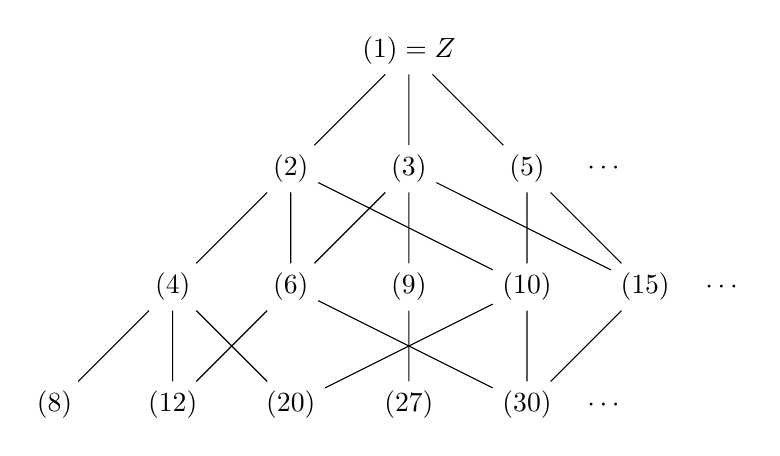
\begin{tikzpicture}
    \begin{scope}[shift={(0,0)}]
        \node (8) at (0,0) {$(8)$};
        \node (4) at (1.5,1.5) {$(4)$};
        \node (2) at (3,3) {$(2)$};
        \node (1) at (4.5,4.5) {$(1) = \ZZ$};

        \node (12) at (1.5,0) {$(12)$};
        \node (6) at (3,1.5) {$(6)$};
        \node (3) at (4.5,3) {$(3)$};

        \node (20) at (3,0) {$(20)$};
        \node (9) at (4.5,1.5) {$(9)$};

        \node (27) at (4.5,0) {$(27)$};

        \node (30) at (6,0) {$(30)$};
        \node (10) at (6,1.5) {$(10)$};
        \node (5) at (6,3) {$(5)$};

        \node (15) at (7.5,1.5) {$(15)$};

        \node (dots1) at (7,3) {$\cdots$};
        \node (dots2) at (8.5,1.5) {$\cdots$};
        \node (dots3) at (7,0) {$\cdots$};

        \draw (1)--(2)--(4)--(8);
        \draw (1)--(3) (1)--(5);
        \draw (2) -- (6) (2) --(10);
        \draw (3) -- (9) -- (27) (3) -- (15) (3) -- (6);
        \draw (5) -- (10) (5) -- (15);
        \draw (4) -- (12) (4) -- (20);
        \draw (6) -- (12) (6) -- (30);
        \draw (10) -- (20) (10) -- (30);
        \draw (15) -- (30);
    \end{scope}
\end{tikzpicture}
\]

\begin{definition}
    \label{def:maximal_prime_ideals}
    Έστω $R$ ένας μεταθετικός δακτύλιος και $I$ ένα ιδεώδες του $R$. Το $I$ ονομάζεται 
    \begin{itemize}
        \item \defn{μεγιστικό} (maximal) αν για κάθε ιδεώδες $J$ του $R$, 
        \[
        I \subseteq J \subseteq R \quad \then \quad J = I \ \ \text{ή} \ \ J = R
        \]
        \item \defn{πρώτο} (prime) αν 
        \[
        ab \in I \quad \then \quad a \in I \ \ \text{ή} \ \ b \in I.
        \]
    \end{itemize}
\end{definition}

Τα μεγιστικά ιδεώδη ενός δακτυλίου είναι τα μεγιστικά στοιχεία του συνδέσμου ιδεωδών του δακτυλίου αυτού με την έννοια της θεωρίας συνόλων. Από την άλλη μεριά, το \emph{λήμμα του Ευκλείδη}, δηλαδή ότι κάθε πρώτος αριθμός που διαιρεί το γινόμενο δύο ακεραίων πρέπει να διαιρεί έναν από τους δύο ακεραίους, έχει ως αποτέλεσμα ένα ιδεώδες $(n)$ του $\ZZ$ να είναι πρώτο αν και μόνο αν το $n$ είναι πρώτος αριθμός. 

Συνεχίζοντας τη συζήτηση για τους δακτύλιους και τα ιδεώδη, ας θυμίσουμε την ιδέα πίσω από την αριθμητική modulo. Παιρνώντας από το $\ZZ$ στο $\ZZ_n$ ουσιαστικά εξισώνουμε το $n$ με το $0$, δηλαδή \textquote{σκοτώνουμε} το $n$ και κατά συνέπεια όλα τα πολλαπλάσιά του, αφήνοντας πίσω τα υπόλοιπα της διαίρεσης των ακεραίων με το $n$. Τα πολλαπλάσια του $n$, όπως είδαμε, αποτελούν ένα ιδεώδες του $\ZZ$. Μπορούμε να μιμηθούμε αυτή τη διαδικασία με έναν αυθαίρετο δακτύλιο $R$ και ένα ιδεώδες $I$ αυτού.

Το σύνολο 
\[
R/I \coloneqq \{r + I : r \in R\}
\]
όπου $r + I \coloneqq \{r + a : a \in I\}$, εφοδιασμένο με τις πράξεις 
\begin{align*}
    \left(r+I\right) + \left(r'+I\right) &\coloneqq (r+r') + I \\
    \left(r+I\right)\cdot\left(r'+I\right) &\coloneqq (rr') + I
\end{align*}
και μηδέν και μονάδα το $0+I$ και $1+I$, αντίστοιχα, ονομάζεται \defn{δακτύλιος πηλίκο} (βλ. \cite[Παράγραφος~8.2.1]{Mpe15}).

\begin{example}
    \label{ex:quotient_ring}
    Έστω $R = \rmT_n(\FF)$ ο δακτύλιος των άνω τριγωνικών $(3\times3)$-πινάκων με στοιχεία σε ένα σώμα $\FF$ και $I$ το ιδεώδες που αποτελείται από όλους τους αυστηρά άνω τριγωνικούς πίνακες. Πώς μοιάζει ο δακτύλιος πηλίκο $R/I$;

    Τα στοιχεία του έχουν την μορφή 
    \begin{align*}
    \begin{pmatrix}
        a & b & c \\
        0 & d & e \\
        0 & 0 & f 
    \end{pmatrix} + I \ 
    &= \begin{pmatrix}
        a & b & c \\
        0 & d & e \\
        0 & 0 & f 
    \end{pmatrix} + 
    \begin{pmatrix}
        0 & \ast & \ast \\ 
        0 & 0 & \ast \\ 
        0 & 0 & 0
    \end{pmatrix} \\ 
    &= 
    \begin{pmatrix}
        a & b + \ast & c + \ast \\
        0 & d & e + \ast \\
        0 & 0 & f 
    \end{pmatrix} \\
    &= 
    \begin{pmatrix}
        a & \ast & \ast \\
        0 & d    & \ast \\
        0 & 0    & f 
    \end{pmatrix}. 
\end{align*}
Με άλλα λόγια, καθορίζονται από τα στοιχεία της διαγωνίου και γι αυτό περνώντας από τον $R$ στον $R/I$ ουσιαστικά \textquote{αγνοούμε} τα στοιχεία πάνω από τη διαγώνιο. 

Οι πράξεις στο $R/I$ έχουν την μορφή 
\begin{align*}
    \begin{pmatrix}
        a & \ast & \ast \\
        0 & b    & \ast \\
        0 & 0    & c \\
    \end{pmatrix}
    +
    \begin{pmatrix}
        x & \ast & \ast \\
        0 & y    & \ast \\
        0 & 0    & z \\
    \end{pmatrix} &=
    \begin{pmatrix}
        a + x & \ast & \ast \\
        0     & b+y  & \ast \\
        0     & 0    & c+z \\
    \end{pmatrix} \\
    \begin{pmatrix}
        a & \ast & \ast \\
        0 & b    & \ast \\
        0 & 0    & c \\
    \end{pmatrix}
    \begin{pmatrix}
        x & \ast & \ast \\
        0 & y    & \ast \\
        0 & 0    & z \\
    \end{pmatrix} &=
    \begin{pmatrix}
        ax & \ast & \ast \\
        0  & by  & \ast \\
        0  & 0    & cz \\
    \end{pmatrix}.
\end{align*}
Με άλλα λόγια, η αριθμητική στο $R/I$ μοιάζει με αυτή στον υποδακτύλιο των διαγώνιων πινάκων. Πράγματι, η απεικόνιση 
\[
\begin{pmatrix}
        a & \ast & \ast \\
        0 & b    & \ast \\
        0 & 0    & c \\
    \end{pmatrix} \ \mapsto 
    \begin{pmatrix}
        a & 0 & 0 \\
        0 & b & 0 \\
        0 & 0 & c \\
    \end{pmatrix}
\]
είναι ισομορφισμός δακτυλίων (γιατί;).

Δεν είναι όλοι οι δακτύλιοι πηλίκο \textquote{κρυμμένοι} υποδακτύλιοι. Για παράδειγμα, ας θεωρήσουμε το εξής ιδεώδες 
\[
J = \left\{
    \begin{pmatrix}
        0 & 0 & a \\
        0 & 0 & 0 \\
        0 & 0 & 0
    \end{pmatrix} : a \in \FF
\right\}
\]
του $R$ και ας δούμε πως μοιάζει ο δακτύλιος πηλίκο $R/J$. 

Τα στοιχεία του έχουν την μορφή 
\[
\begin{pmatrix}
    a & b & \ast \\ 
    0 & c & d \\ 
    0 & 0 & e \\ 
\end{pmatrix}
\]
και ο πολλαπλασιασμός γίνεται 
\[
\begin{pmatrix}
    a & b & \ast \\ 
    0 & c & d \\ 
    0 & 0 & e \\ 
\end{pmatrix}
\begin{pmatrix}
    v & w & \ast \\ 
    0 & x & y \\ 
    0 & 0 & z \\ 
\end{pmatrix} = 
\begin{pmatrix}
    av & aw + bx & a\ast + \textcolor{burntorange}{by} + \ast{z} \\ 
    0 & cx & cy + dz \\ 
    0 & 0 & ez
\end{pmatrix}.
\]
Παρατηρούμε λοιπόν ότι \emph{δεν} μπορούμε να αντικαταστίσουμε το στοιχείο της θέσης $(1,3)$ με ένα αυθαίρετο στοιχείο του $\FF$ όπως κάναμε στην περίπτωση του $R/I$. Άρα, ο δακτύλιος $R/J$ δεν \textquote{μοιάζει} με κάποιον υποδακτύλιο του $R$ και στην περίπτωση αυτή περνώντας από τον $R$ στον $R/I$ προκύπτει ένας \textquote{καινούργιος} δακτύλιος.
\end{example}

\begin{theorem}{\rm(Θεωρήματα Ισομορφισμών)}
    \label{thm:isomorphism_theorems}
    \leavevmode
    \begin{itemize}
        \item[(1)] Αν $\phi : R \to S$ είναι ένας ομομορφισμός δακτυλίων, τότε $R/\ker\phi \cong \phi(R)$.
        \item[(2)] Αν $I$ και $J$ είναι ιδεώδη κάποιου δακτύλιου, τότε $I/(I\cap{J}) \cong (I+J)/J$.
        \item[(3)] Αν $I$ και $J$ είναι δύο ιδεώδη ενός δακτύλιου $R$ τέτοια ώστε $J \subseteq I$, τότε $\frac{R/J}{I/J} \cong R/I$.
        \item[(4)] Υπάρχει μια αμφιμονοσήμαντη αντιστοιχία μεταξύ των ιδεωδών του $R/I$ και των ιδεωδών του $R$ τα οποία περιέχουν το ιδεώδες $I$.
    \end{itemize}
\end{theorem}

Για μια λεπτομερή συζήτηση του Θεωρήματος \ref{thm:isomorphism_theorems} παραπέμπουμε στην Ενότητα 8.3 του \cite{Mpe15}. Ας προσπαθήσουμε να \textquote{δούμε} τι μας πληροφορούν τα τέσσερα θεωρήματα ισομορφισμών.
\begin{itemize}
    \item Το πρώτο θεώρημα ισομορφιμού μας πληροφορεί ότι κάθε ομομορφισμός δακτυλίων $\phi : R \to S$ \textquote{κρύβει} εντός του έναν ισομορφισμό $\tilde{\phi} : R/\rmKer(\phi) \to \phi(R)$
    \[
    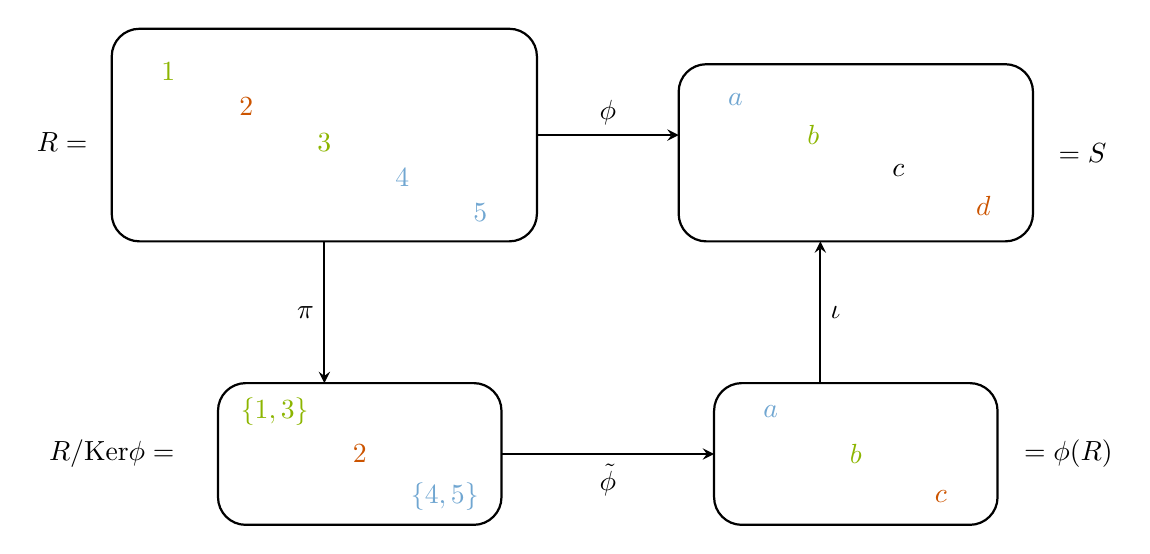
\begin{tikzpicture}[>=stealth,scale=.9]

    % =====================
    % Upper left box
    % =====================
    \begin{scope}[shift={(0,4)}]
    \draw[rounded corners=10pt, thick] (0,0) rectangle (6,3);

    \node at (0.8,2.4) {$\mathcolor{applegreen}{1}$};
    \node at (1.9,1.9) {$\mathcolor{burntorange}{2}$};
    \node at (3.0,1.4) {$\mathcolor{applegreen}{3}$};
    \node at (-.7,1.4) {$R =$};
    \node at (4.1,0.9) {$\mathcolor{iceberg}{4}$};
    \node at (5.2,0.4) {$\mathcolor{iceberg}{5}$};
    \end{scope}

    % =====================
    % Upper right box
    % =====================
    \begin{scope}[shift={(8,4)}]
    \draw[rounded corners=10pt, thick] (0,0) rectangle (5,2.5);

    \node at (0.8,2.0) {$\mathcolor{iceberg}{a}$};
    \node at (1.9,1.5) {$\mathcolor{applegreen}{b}$};
    \node at (5.7,1.25) {$= S$};
    \node at (3.1,1.0) {$c$};
    \node at (4.3,0.5) {$\mathcolor{burntorange}{d}$};
    \end{scope}

    % =====================
    % Lower left box
    % =====================
    \begin{scope}[shift={(1.5,0)}]
    \draw[rounded corners=10pt, thick] (0,0) rectangle (4,2);

    \node at (0.8,1.6) {$\mathcolor{applegreen}{\{1,3\}}$};
    \node at (2.0,1.0) {$\mathcolor{burntorange}{2}$};
    \node at (-1.5,1.0) {$R/\rmKer\phi =$};
    \node at (3.2,0.4) {$\mathcolor{iceberg}{\{4,5\}}$};
    \end{scope}

    % =====================
    % Lower right box
    % =====================
    \begin{scope}[shift={(8.5,0)}]
    \draw[rounded corners=10pt, thick] (0,0) rectangle (4,2);

    \node at (0.8,1.6) {$\mathcolor{iceberg}{a}$};
    \node at (2.0,1.0) {$\mathcolor{applegreen}{b}$};
    \node at (5,1.0) {$= \phi(R)$};
    \node at (3.2,0.4) {$\mathcolor{burntorange}{c}$};
    \end{scope}

    % =====================
    % Arrows
    % =====================
    \draw[->, thick] (6,5.5) -- node[above] {$\phi$} (8,5.5);
    \draw[->, thick] (3,4) -- node[left] {$\pi$} (3,2);
    \draw[->, thick] (5.5,1) -- node[below] {$\tilde{\phi}$} (8.5,1);
    \draw[->, thick] (10,2) -- node[right] {$\iota$} (10,4);

    \end{tikzpicture}
    \]
    \textquote{περνώντας} μέσα από την κανονική προβολή $\pi : R \to R/\rmKer\phi$ και τον κανονικό εγκλεισμό $\iota : \phi(R) \to S$ έτσι ώστε 
    \[
    \phi = \iota \circ \tilde{\phi} \circ \pi.
    \]

    \item Το τέταρτο θεώρημα ισομορφισμού μας πληροφορεί ότι ο σύνδεσμος ιδεωδών του $R/I$ ταυτίζεται με το κομμάτι του συνδέσμου ιδεωδών του $R$ που βρίσκεται (ασθενώς) πάνω από το $I$. Για παράδειγμα, για $R = \ZZ$ και $I = (12)$, ο σύδεσμος ιδεωδών του $R/I$ είναι 
\[
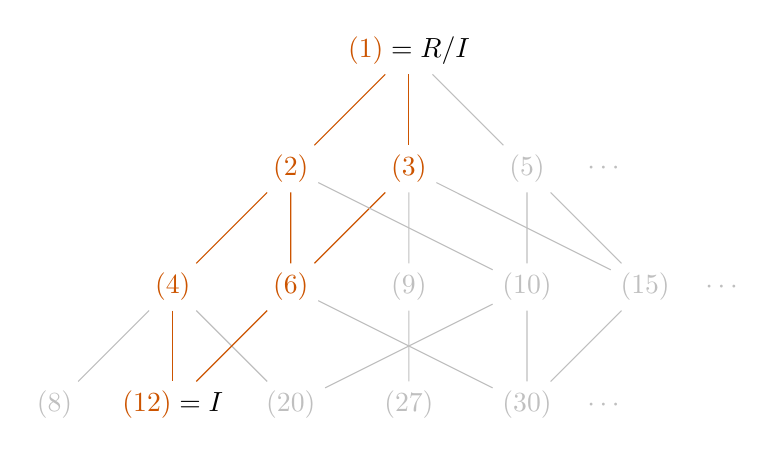
\begin{tikzpicture}
    \begin{scope}[shift={(0,0)}]
        \node[color=gray!50] (8) at (0,0) {$(8)$};
        \node (4) at (1.5,1.5) {$\mathcolor{burntorange}{(4)}$};
        \node (2) at (3,3) {$\mathcolor{burntorange}{(2)}$};
        \node (1) at (4.5,4.5) {$\mathcolor{burntorange}{(1)} = R/I$};

        \node (12) at (1.5,0) {$\mathcolor{burntorange}{(12)} = I$};
        \node (6) at (3,1.5) {$\mathcolor{burntorange}{(6)}$};
        \node (3) at (4.5,3) {$\mathcolor{burntorange}{(3)}$};

        \node[color=gray!50] (20) at (3,0) {$(20)$};
        \node[color=gray!50] (9) at (4.5,1.5) {$(9)$};

        \node[color=gray!50] (27) at (4.5,0) {$(27)$};

        \node[color=gray!50] (30) at (6,0) {$(30)$};
        \node[color=gray!50] (10) at (6,1.5) {$(10)$};
        \node[color=gray!50] (5) at (6,3) {$(5)$};

        \node[color=gray!50] (15) at (7.5,1.5) {$(15)$};

        \node[gray!50] (dots1) at (7,3) {$\cdots$};
        \node[gray!50] (dots2) at (8.5,1.5) {$\cdots$};
        \node[gray!50] (dots3) at (7,0) {$\cdots$};

        \draw[burntorange] (1)--(2)--(4);
        \draw[gray!50] (4) -- (8);
        \draw[burntorange] (1)--(3);
        \draw[gray!50] (1)--(5);
        \draw[burntorange] (2) -- (6) (3) -- (6);
        \draw[gray!50] (2) --(10);
        \draw[gray!50] (3) -- (9) -- (27) (3) -- (15);
        \draw[gray!50] (5) -- (10) (5) -- (15);
        \draw[burntorange] (4) -- (12);
        \draw[gray!50] (4) -- (20);
        \draw[burntorange] (6) -- (12);
        \draw[gray!50] (6) -- (30);
        \draw[gray!50] (10) -- (20) (10) -- (30);
        \draw[gray!50] (15) -- (30);
    \end{scope}
\end{tikzpicture}
\]

\item Το δεύτερο θεώρημα ισομορφισμού μας πληροφορεί ότι το \textquote{διάστημα} του συνδέσμου ιδεωδών του $R$ που βρίσκεται μεταξύ των $I\cap J$ και $Ι$ ταυτίζεται με αυτό που βρίσκεται μεταξύ των $J$ και $I+J$. Για παράδειγμα, για $R = \ZZ, I = (4)$ και $J = (15)$ έχουμε 
\[
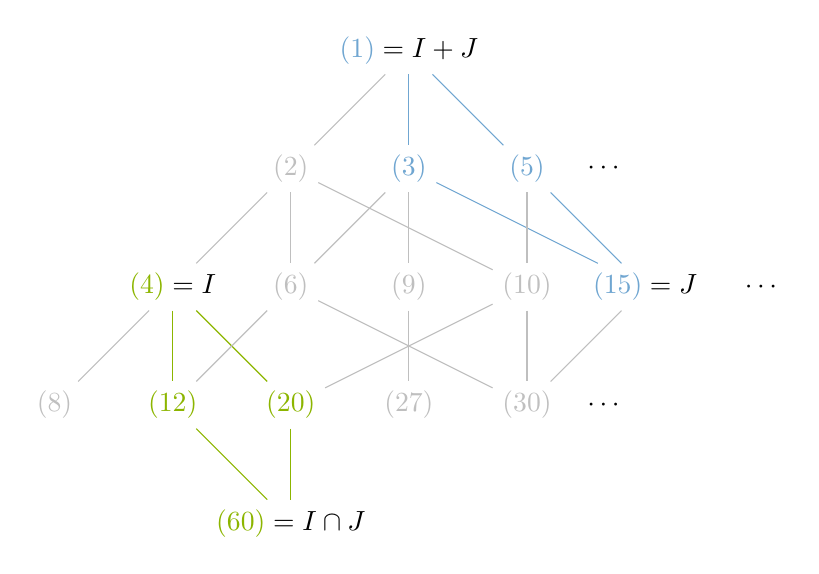
\begin{tikzpicture}
    \begin{scope}[shift={(0,0)}]
        \node[gray!50] (8) at (0,0) {$(8)$};
        \node (4) at (1.5,1.5) {$\mathcolor{applegreen}{(4)} = I$};
        \node[gray!50] (2) at (3,3) {$(2)$};
        \node (1) at (4.5,4.5) {$\mathcolor{iceberg}{(1)} = I+J$};

        \node (12) at (1.5,0) {$\mathcolor{applegreen}{(12)}$};
        \node[gray!50] (6) at (3,1.5) {$(6)$};
        \node (3) at (4.5,3) {$\mathcolor{iceberg}{(3)}$};

        \node (20) at (3,0) {$\mathcolor{applegreen}{(20)}$};
        \node (60) at (3,-1.5) {$\mathcolor{applegreen}{(60)} = I\cap{J}$};
        \node[gray!50] (9) at (4.5,1.5) {$(9)$};

        \node[gray!50] (27) at (4.5,0) {$(27)$};

        \node[gray!50] (30) at (6,0) {$(30)$};
        \node[gray!50] (10) at (6,1.5) {$(10)$};
        \node (5) at (6,3) {$\mathcolor{iceberg}{(5)}$};

        \node (15) at (7.5,1.5) {$\mathcolor{iceberg}{(15)} = J$};

        \node (dots1) at (7,3) {$\cdots$};
        \node (dots2) at (9,1.5) {$\cdots$};
        \node (dots3) at (7,0) {$\cdots$};

        \draw[gray!50] (1)--(2);
        \draw[gray!50] (2) --(4);
        \draw[gray!50] (4)--(8);
        \draw[iceberg] (1)--(3);
        \draw[iceberg] (1)--(5);
        \draw[gray!50] (2) -- (6);
        \draw[gray!50] (2) --(10);
        \draw[gray!50] (3) -- (9);
        \draw[gray!50] (9) -- (27);
        \draw[iceberg] (3) -- (15);
        \draw[gray!50] (3) -- (6);
        \draw[gray!50] (5) -- (10);
        \draw[iceberg] (5) -- (15);
        \draw[applegreen] (4) -- (12); 
        \draw[applegreen] (4) -- (20);
        \draw[applegreen] (12) -- (60);
        \draw[applegreen] (20) -- (60);
        \draw[gray!50] (6) -- (12); 
        \draw[gray!50] (6) -- (30);
        \draw[gray!50] (10) -- (20); 
        \draw[gray!50] (10) -- (30);
        \draw[gray!50] (15) -- (30);
    \end{scope}
\end{tikzpicture}
\]

\item Το τρίτο θεώρημα ισομορφιμού μας πληροφορεί ότι ο σύνδεσμος ιδεωδών του $R/I$ είναι ίδιος με την \textquote{συστολή} του συνδέσμου ιδεωδών του $R/J$ ως προς το σύνδεσμο ιδεωδών του $I/J$. Για παράδειγμα, για $R=\ZZ, I=(6)$ και $J=(30)$ έχουμε 
\[
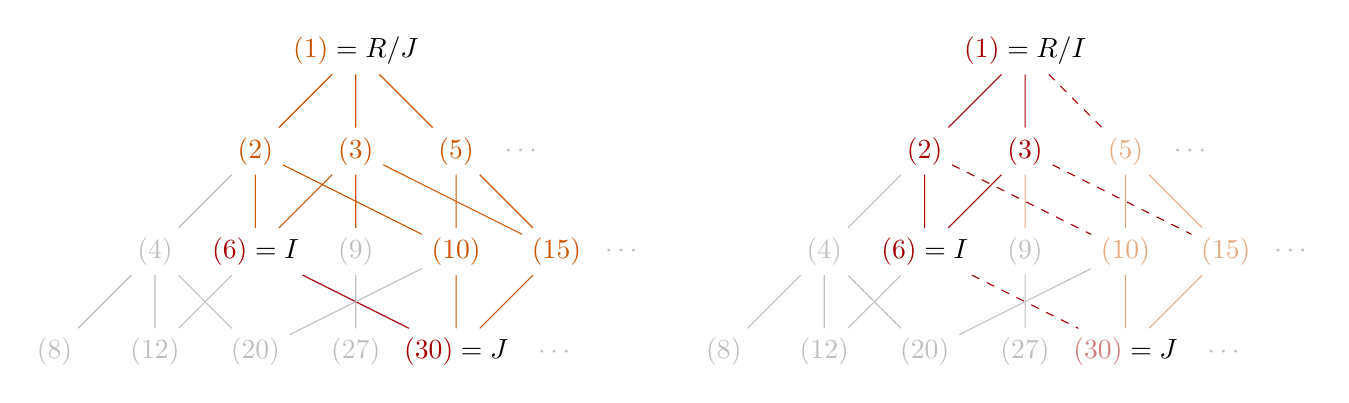
\begin{tikzpicture}[scale=.85]
    \begin{scope}[shift={(0,0)}]
        \node[gray!50] (8) at (0,0) {$(8)$};
        \node[gray!50] (4) at (1.5,1.5) {$(4)$};
        \node (2) at (3,3) {$\mathcolor{burntorange}{(2)}$};
        \node (1) at (4.5,4.5) {$\mathcolor{burntorange}{(1)} = R/J$};

        \node[gray!50] (12) at (1.5,0) {$(12)$};
        \node (6) at (3,1.5) {$\mathcolor{darkcandyapplered}{(6)} = I$};
        \node (3) at (4.5,3) {$\mathcolor{burntorange}{(3)}$};

        \node[gray!50] (20) at (3,0) {$(20)$};
        \node[gray!50] (9) at (4.5,1.5) {$(9)$};

        \node[gray!50] (27) at (4.5,0) {$(27)$};

        \node (30) at (6,0) {$\mathcolor{darkcandyapplered}{(30)} = J$};
        \node (10) at (6,1.5) {$\mathcolor{burntorange}{(10)}$};
        \node (5) at (6,3) {$\mathcolor{burntorange}{(5)}$};  

        \node (15) at (7.5,1.5) {$\mathcolor{burntorange}{(15)}$};

        \node[gray!50] (dots1) at (7,3) {$\cdots$};
        \node[gray!50] (dots2) at (8.5,1.5) {$\cdots$};
        \node[gray!50] (dots3) at (7.5,0) {$\cdots$};

        \draw[burntorange] (1)--(2);
        \draw[gray!50] (2) --(4);
        \draw[gray!50] (4)--(8);
        \draw[burntorange] (1)--(3);
        \draw[burntorange] (1)--(5);
        \draw[burntorange] (2) -- (6);
        \draw[burntorange] (2) --(10);
        \draw[burntorange] (3) -- (9);
        \draw[gray!50] (9) -- (27);
        \draw[burntorange] (3) -- (15);
        \draw[burntorange] (3) -- (6);
        \draw[burntorange] (5) -- (10);
        \draw[burntorange] (5) -- (15);
        \draw[gray!50] (4) -- (12); 
        \draw[gray!50] (4) -- (20);
        \draw[gray!50] (6) -- (12); 
        \draw[darkcandyapplered] (6) -- (30);
        \draw[gray!50] (10) -- (20); 
        \draw[burntorange] (10) -- (30);
        \draw[burntorange] (15) -- (30);
    \end{scope}
    \begin{scope}[shift={(10,0)}]
        \node[gray!50] (8) at (0,0) {$(8)$};
        \node[gray!50] (4) at (1.5,1.5) {$(4)$};
        \node (2) at (3,3) {$\mathcolor{darkcandyapplered}{(2)}$};
        \node (1) at (4.5,4.5) {$\mathcolor{darkcandyapplered}{(1)} = R/I$};

        \node[gray!50] (12) at (1.5,0) {$(12)$};
        \node (6) at (3,1.5) {$\mathcolor{darkcandyapplered}{(6)} = I$};
        \node (3) at (4.5,3) {$\mathcolor{darkcandyapplered}{(3)}$};

        \node[gray!50] (20) at (3,0) {$(20)$};
        \node[gray!50] (9) at (4.5,1.5) {$(9)$};

        \node[gray!50] (27) at (4.5,0) {$(27)$};

        \node (30) at (6,0) {$\mathcolor{darkcandyapplered!50}{(30)} = J$}; 
        \node (10) at (6,1.5) {$\mathcolor{burntorange!50}{(10)}$};
        \node (5) at (6,3) {$\mathcolor{burntorange!50}{(5)}$};
        

        \node (15) at (7.5,1.5) {$\mathcolor{burntorange!50}{(15)}$};
        
        \node[gray!50] (dots1) at (7,3) {$\cdots$};
        \node[gray!50] (dots2) at (8.5,1.5) {$\cdots$};
        \node[gray!50] (dots3) at (7.5,0) {$\cdots$}; 

        \draw[darkcandyapplered] (1)--(2);
        \draw[gray!50] (2) --(4);
        \draw[gray!50] (4)--(8);
        \draw[darkcandyapplered] (1)--(3);
        \draw[darkcandyapplered,dashed] (1)--(5);
        \draw[darkcandyapplered] (2) -- (6);
        \draw[darkcandyapplered,dashed] (2) --(10);
        \draw[burntorange!50] (3) -- (9);
        \draw[gray!50] (9) -- (27);
        \draw[darkcandyapplered,dashed] (3) -- (15);
        \draw[darkcandyapplered] (3) -- (6);
        \draw[burntorange!50] (5) -- (10);
        \draw[burntorange!50] (5) -- (15);
        \draw[gray!50] (4) -- (12); 
        \draw[gray!50] (4) -- (20);
        \draw[gray!50] (6) -- (12); 
        \draw[darkcandyapplered,dashed] (6) -- (30);
        \draw[gray!50] (10) -- (20); 
        \draw[burntorange!50] (10) -- (30);
        \draw[burntorange!50] (15) -- (30);
    \end{scope}
\end{tikzpicture}
\]
\end{itemize}

Έχοντας κατά νου ότι τα σώματα δεν έχουν γνήσια, μη τετριμμένα ιδεώδη, κοιτάζοντας τον σύνδεσμο ιδεδών του $\ZZ$ μπορούμε να επιβεβαιώσουμε (οπτικά) τις ακόλουθες ισοδυναμίες 
\begin{itemize}
    \item το $\ZZ/(n)$ είναι σώμα 
    \item το $(n)$ είναι μεγιστικό ιδεώδες 
    \item ο $n$ είναι πρώτος,
\end{itemize}
όπου είδαμε παραπάνω ότι το τελευταίο είναι ισοδύναμο με το $(n)$ να είναι πρώτο ιδεώδες. Γενικότερα, ισχύει το εξής.

\begin{proposition}
    \label{prop:maximal_ideals_characterization}
    Έστω $R$ ένας μεταθετικός δακτύλιος και $I$ ιδεώδες του $R$. Το $I$ είναι μεγιστικό αν και μόνο αν ο $R/I$ είναι σώμα.
\end{proposition}

Η απόδειξη της Πρότασης \ref{prop:maximal_ideals_characterization} έπεται άμεσα από το τέταρτο θεώρημα ισομορφισμού (γιατί;). Στην περίπτωση του δακτυλίου των ακεραίων οι έννοιες του μεγιστικού και του πρώτου ιδεώδους ταυτίζονται. Γενικότερα, από την Πρόταση \ref{prop:maximal_ideals_characterization} έπεται ότι κάθε μεγιστικό ιδεώδες είναι πρώτο (γιατί;). Το αντίστροφο δεν ισχύει, καθώς για παράδειγμα το ιδεώδες\footnote{Θα μελετήσουμε πιο αναλυτικά τους πολυωνυμικούς δακτυλίους στην Ενότητα 3.} $(x)$ στο $\ZZ[x]$ είναι πρώτο, αλλά όχι μεγιστικό διότι το $\ZZ[x]/(x) \cong \ZZ$ είναι ακέραια περιοχή, όπως δείχνει η επόμενη πρόταση.

\begin{proposition}
    \label{prop:prime_ideals_characterization}
    Έστω $R$ ένας μεταθετικός δακτύλιος και $I$ ιδεώδες του $R$. Το $I$ είναι πρώτο αν και μόνο αν ο $R/I$ είναι ακέραια περιοχή.
\end{proposition}

\begin{thebibliography}{99}
    \bibitem{Mpe15}
    Α. Μπελιγιάννης, 
    \textit{Μια Εισαγωγή στη Βασική Άλγεβρα},
    Κάλλιπος, 2015. (διαθέσιμο \href{https://dx.doi.org/10.57713/kallipos-547}{εδώ})
\end{thebibliography}
\end{document}